\documentclass[conference]{IEEEtran}

\usepackage{tikz}

\usepackage[slovene]{babel}

% correct bad hyphenation here
\hyphenation{}

\begin{document}
	
	\title{Implementacija spletnega pajka}
	
	\author{Skupina \textbf{DOMACI-NJOKI}: Niki Bizjak, Bojan Vrangeloski, Uroš Škrjanc}


	
	\maketitle
	
	\begin{abstract}
		V poročilu o seminarski smo opisali strukturo našega spletnega pajka, njegovo delovanje in rezultate, ki smo jih dobili pri preizkušanju pajka.
	\end{abstract}
	
	\IEEEpeerreviewmaketitle
	
	\section{Uvod}
	
	Za prvo seminarsko nalogo pri predmetu Iskanje in ekstrakcija podatkov s spleta smo implementirali spletnega pajka, ki je obiskal in v lokalno podatkovno bazo prenesel vsebino spletnih strani na štirih spletnih mestih (\texttt{gov.si}, \texttt{evem.gov.si}, \texttt{e-uprava.gov.si}, \texttt{e-prostor.gov.si}). V nadaljevanju poročila smo opisali strukturo in delovanje našega pajka, predstavili rezultate naše naloge in težave, na katere smo naleteli tekom dela.
	
	\section{Struktura pajka}
	
	Pajka smo izdelali v programskem jeziku Python. Strukturno je pajek razdeljen na tri med seboj povezane komponente, ki so v programski kodi definirani kot objekti: razvrščevalnik, pajek in shramba.
	
	
	\begin{figure}[h]
		\centering
		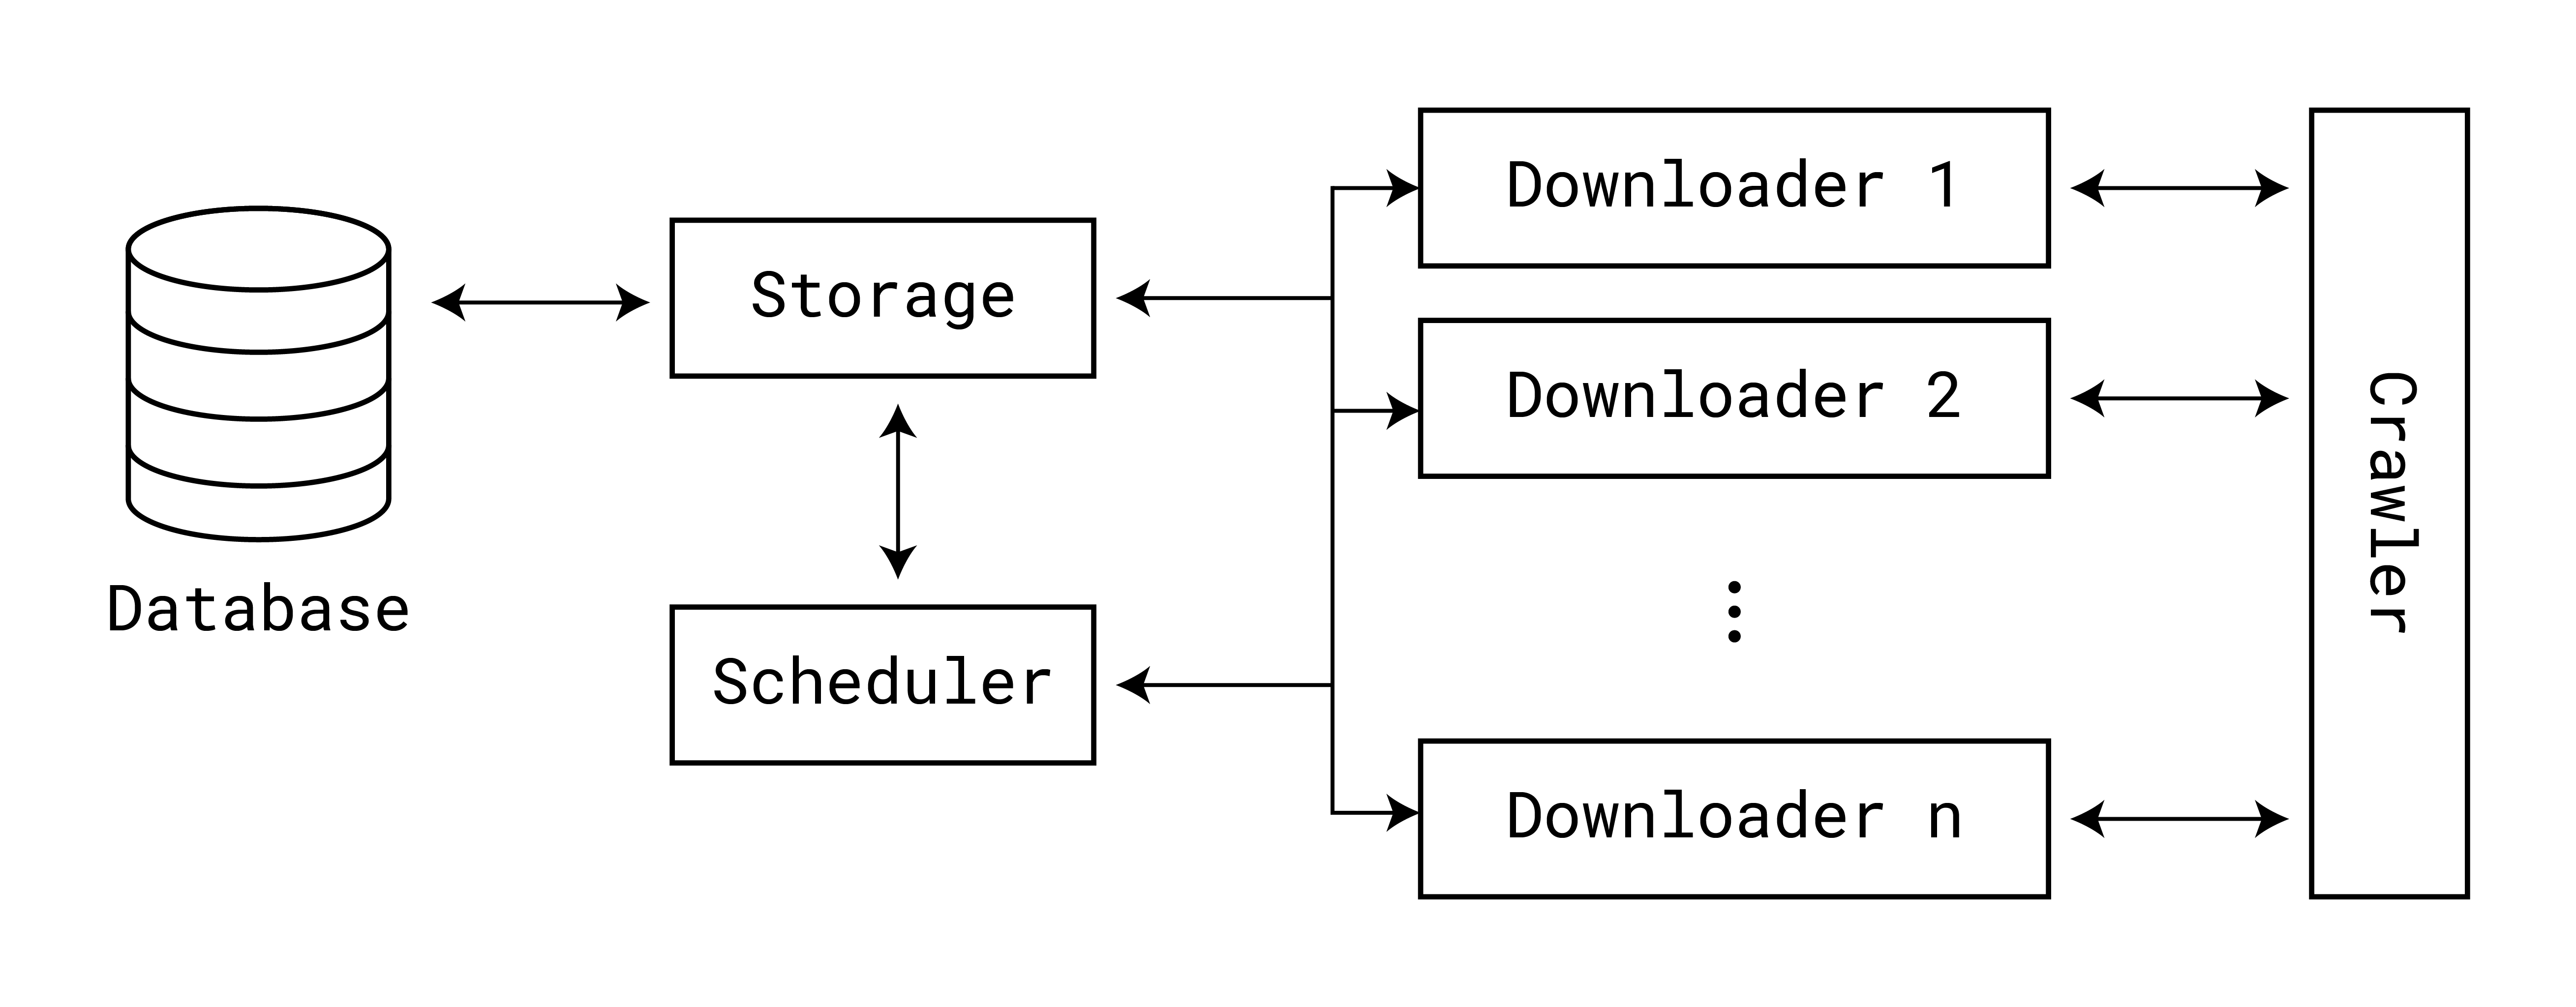
\includegraphics[width=.9\linewidth]{images/arhitecture}
		\caption{Arhitektura implementiranega spletnega pajka}
	\end{figure}

	\subsection{Razvrščevalnik}

	Razvrščevalnik (ang. scheduler) URL naslovov je implementiran kot podatkovna vrsta, do katere lahko obenem dostopa več različnih niti. Skrbi za seznam naslovov, ki jih mora naš pajek še obiskati in za etično delovanje pajka - zagotoviti je potrebno, da pajek do istega strežnika ne dostopa bolj pogosto, kot to strežnik dovoljuje.
	
	Ob dodajanju novega URL naslova v vrsto, razvrščevalnik preveri, ali je bil ta URL naslov že prenesen. Prav tako zna iz URL naslova prebrati domeno, pridobiti IP naslov strežnika s to domeno in prenesti datoteko \texttt{robots.txt}.
	
	Razvrščevalnik hrani seznam IP naslovov in čas zadnjega dostopa do določenega strežnika. Za vsak IP naslov vzdržuje vrsto URL naslovov, ki jih je potrebno še prenesti. Ko nit pajka od razvrščevalnika zahteva URL naslov, ta preveri kateri izmed strežnikov je bil obiskan najprej in iz vrste za ta strežnik vzame prvi URL naslov tega strežnika. Ko nit pridob URL naslov za prenos, se v razvrščevalniku IP naslov, ki pripada tej domeni, zaklene in se odklene šele po tem, ko nit razvrščevalniku sporoči, da je bil prenos uspešen.
	
	Pri dodajanju URL naslovov v razvrščevalnik, najprej preverimo, ali je bila stran že obiskana. Če še ni bila, iz domene pridobimo IP naslov strežnika in URL shranimo na konec vrste z ustreznim IP naslovom. Implementiran pajek tako izvaja preiskovanje v širino (angl. breadth-first search) za posamezen IP naslov strežnika. Na tak način zagotovimo, da bo pajek v primernem času zagotovo obiskal vse strani, v danem trenutku pa pajek dostopa do strežnikov z različnimi IP naslovi, kar je v skladu z dogovorjenimi etičnimi načeli.
	
	\subsection{Pajek}
	
	Ob zagonu, pajek (ang. crawler) zažene več niti, vsaka od njih pa ima nalogo, da iz razvrščevalnika URL naslovov pridobi naslov, prenese stran in shrani podatke v podatkovno bazo. Pridobivanje vsebine strani izvajamo v dveh korakih:
	
	\begin{itemize}
		\item Najprej na strežnik izvedemo \texttt{HTTP HEAD} zahtevek. Na tak način pridobimo statusno kodo strežnika in morebitne preusmeritve med stranmi. Pajek v tem koraku tudi preveri kakšen je \texttt{Content-Type} strani. Če je vsebina strani \texttt{HTML}, potem nadaljujemo s prenosom, v nasprotnem primeru pa v tabelo \texttt{page\_data} vstavimo ustrezen vnos s tipom datoteke.
		\item S pomočjo Selenium brskalnika obiščemo stran. Če pri prenašanju strani pride do prekoračitve vnaprej določenega časa, z obiskom prekinemo in URL naslov ponovno dodamo na konec vrste.
	\end{itemize}

	Pajek po prenosu strani s spleta izvede še naslednje korake procesiranja:
	\begin{itemize}
		\item Iz HTML vsebine strani izračuna razpršilno vrednost (angl. hash) in preveri, ali stran z enako vrednostjo v bazi že obstaja. V tem primeru, se v bazi URL naslov označi kot duplikat.
		\item Na strani poiščemo vse slike in jih vstavimo v tabelo \texttt{image} v podatkovni bazi.
		\item Na strani se poiščejo vse hiperpovezave. Razvrščevalnik za vsako hiperpovezavo najprej izračuna njeno kanonizirano obliko in skuša na podlagi poti v naslovu ugotoviti, kakšne vrste je datoteka. V primeru, da ima datoteka ustrezno končnico (npr. \texttt{.pdf}, \texttt{.docx}, ...), takega URL naslova ne dodamo v vrsto, temveč ustvarimo nov zapis v tabeli \texttt{page\_data} v podatkovni bazi.
		\item Pridobljene hiperpovezave dodamo v razvrščevalnik.
	\end{itemize}
	
	\subsection{Shramba}
	
	Shramba (ang. storage) je del pajka, ki skrbi za vpis zbranih podatkov in vsebin v relacijsko bazo podatkov. Baza je postavljena v okolju PostgreSQL, strukturi baze, ki je bila predlagana v projektu, pa smo v tabeli \texttt{page} dodali še polje \texttt{page hash}, v katerem se shranjuje hash vrednost, izračunana z MD5 algoritmom. Hash vrednost smo shranjevali za preverjanje, ali spletna stran z določeno vsebino že obstaja. 
	
	Za vpisovanje, popravljanje in izpis podatkov iz podatkovne baze smo sprogramirali 25 funkcij, vsaka od teh funkcij zaklene dostop do podatkovne baze, da ne bi prišlo do pomanjkljivih ali večkratnih vpisov vsebin.
	
	\section{Delo na projektu}
	
	Kar se tiče samega dela na projektu, je bilo najtežje uskladiti večnitno delovanje pajka in čakanje pri pošiljanju zahtev za spletne strani, tako da pajek deluje stabilno in hkrati v skladu z etičnimi načeli. Vsaka takšna zahteva usklajeno delovanje tako med večimi nitmi samega pajka, kot tudi med vsemi komponentami, apliciranimi v pajku.
	Na težave smo naleteli tudi pri uporabi gonilnika Geckodriver za brskanje v ozadju po spletnih straneh. Če je pajek prišel do strani, kjer je uporabnik moral izbrati osebno digitalno potrdilo, se je, ne glede na nastavljen 10 sekundni timeout, nit ustavila. To smo rešili tako, da smo Geckodriver zamenjali z gonilnikom za brskalnik Chrome, ki je potem delal veliko bolje.
	
	\section{Rezultati}
	Naš spletni pajek je v 20 urah zbral podatke o 221 spletnih mestih, 52.146 spletnih straneh, 34.118 dokumentih in 434.080 slikovnih datotekah. V bazo som ujeli tudi 6 spletnih mest in 3.396 strani, ki so imele preusmeritev s strani gov.si domene in ne gostujejo na tej domeni. Glede na to, da gre za kar veliko količino podatkov, predvsem s kvantitativnega vidika, smatramo, da je delovanje pajka zadovoljivo. Tudi same podatke smo uspeli s spletnih mest pridobiti tako, da so primerni za nadaljnjo uporabo, kar se nam zdi pomembno za to nalogo. Je pa, seveda, tudi še nekaj prostora za izboljšave, ki bi jih lahko, če bi imeli na razpolago nekaj več časa, tudi implementirali.
	
	V spodnji tabeli navajamo rezultate.
	
		

\begin{flushleft}
\begin{tabular}{ |l|l|l|l|l| } 
 \hline
  &  gov.si & evem.gov.si & e-uprava.gov.si & e-prostor.gov.si  \\
 \hline
 Število spletnih mest &  215 & 1 & 1 & 4  \\ 
 \hline
 Število spletnih strani &  47631 & 365 & 3020 & 1130  \\  
 \hline
 Število dvojnikov strani &  10636 & 287 & 56 & 412 \\
 \hline
 Število vseh dokumentov &  33122 & 27 & 9 & 960 \\
 \hline
 Število PDF dokumentov &  23998 & 6 & 8 & 905 \\
 \hline
 Število DOC dokumentov &  2498 & 15 & 0 & 39 \\
 \hline
 Število DOCX dokumentov &  6197 & 6 & 1 & 12 \\
 \hline
 Število PPT dokumentov &  176 & 0 & 0 & 1 \\
 \hline
 Število PPTX dokumentov &  253 & 0 & 0 & 3 \\
 \hline
 Število slik &  425016 & 563 & 3199 & 5302 \\
 \hline
 Povprečno število slik na stran &  9 & 1,5 & 1 & 4,6 \\
 \hline
 Povprečno število dokumentov na stran &  0,8 & 0,08 & 0,01 & 0,9 \\
 \hline
\end{tabular}
\end{flushleft}


	
	

	
	
	
	% \bibliographystyle{IEEEtran}
	% \bibliography{}
	
\end{document}
